%!TEX root = foo-thesis.tex

\chapter{Einleitung}
\label{chap:intro}

\section{Projektüberblick}

3D-Punktwolken können mit Hilfe von Laserscannern oder photogrammetrischen Verfahren mit vergleichsweise geringem Aufwand zeit- und kosteneffizient erzeugt werden. Sie stellen ein häufig bis auf wenige Millimeter genaues Modell der realen Welt dar, welches außerdem Informationen wie zum Beispiel die Farbe des abgebildeten realen Objekts beinhalten kann. Entsprechend kann das Modell, je nach Detailgrad und Verfügbarkeit solcher Attribute, genutzt werden, um Erkenntnisse über Gegebenheiten der realen Welt zu erlangen. So kann zum Beispiel die Planarität, nachdem sie mithilfe der Koordinaten der Punkte berechnet wurde, Auskunft über die Oberflächenstruktur der 3D-Punktwolke geben. Für die Extraktion dieser Informationen werden allerdings auch geeignete Algorithmen benötigt, wie beispielsweise geometrische Verfahren zur Klassifizierung von Bodenpunkten. Besonders wichtig ist dabei, dass diese Algorithmen effizient sind, um die großen Datenmengen, die beim Erstellen einer 3D-Punktwolke entstehen, verarbeiten zu können. Es existieren jedoch auch Problemstellungen, welche algorithmisch nur vergleichsweise ineffizient gelöst werden können, sodass sich beispielsweise für die semantische Segmentierung einer 3D-Punktwolke - also der Bestimmung, zu welcher Objektklasse ein Punkt gehört - \textit{Machine-Learning}-Ansätze anbieten. Für diese Fälle wird allerdings generell leistungsfähige Hardware - insbesondere moderne CPUs, GPUs sowie RAM in ausreichender Menge - und viel Rechenzeit benötigt. Insofern gibt es Anwendungsfälle, die nur dann sinnvoll umgesetzt werden können, wenn der verwendete Algorithmus in ausreichender Form skalierbar ist. \\\\
Weiterhin sind viele der Algorithmen sehr komplex, um auch verschiedene Arten von Punktwolken mit unterschiedlichen Charakteristika wie ihrer Dichte, aber auch Pro-Punkt-Eigenschaften wie der Intensität und Farbwerten sinnvoll verarbeiten zu können. Dies setzt voraus, dass der Anwender über ein tiefgreifendes Verständnis sowohl vom Aufbau der 3D-Punktwolken selbst als auch von verfügbaren Algorithmen und deren Parametern verfügt. Daraus folgt jedoch, dass Nutzer mit weniger fundiertem Fachwissen nur begrenzte Möglichkeiten haben, 3D-Punktwolken vor allem für komplexere Anwendungsfälle gewinnbringend zu nutzen. \\\\
Um diese Probleme zu lösen, wurde im Projekt eine Plattform entwickelt, die sowohl die nötige Skalierbarkeit zur Anwendung hochkomplexer Algorithmen und \textit{Deep-Learning}-Verfahren bietet als auch eine entsprechend hohe Nutzerfreundlichkeit sicherstellt. Um dem Nutzer die Arbeit mit der Plattform besonders einfach zu machen, wurden im Projekt spezielle Verfahren entwickelt, um die verschiedenen Algorithmen auf die in der Plattform hochgeladenen 3D-Punktwolken anzupassen. So können potenziell auch sehr komplexe Analysen, wie beispielsweise die Erkennung von Straßenschäden, für ein weites Spektrum an 3D-Punktwolken ausgeführt werden, die sich in der Art ihrer Aufnahme, in ihren geometrischen Eigenschaften oder in ihrer räumlichen Ausdehnung unterscheiden.

\section{Terminologie}

Im Nachfolgenden sollen wichtige Begriffe kurz erklärt werden.

\subsection*{3D-Punktwolke}
Der Begriff 3D-Punktwolke beschreibt eine ungeordnete Menge von Punkten in einem dreidimensionalen Raum. Zusätzlich zu den Koordinaten, die die Position im Raum beschreiben, werden bei der Erstellung einer 3D-Punktwolke häufig noch weitere Attribute wie der Intensitäts- oder Farbwert aufgenommen. Des Weiteren lassen sich über gängige Algorithmen zusätzliche punktspezifische Eigenschaften wie die Oberflächennormale \citep{Mitra.Nguyen-2003} oder ein Krümmungswert \citep{Ho.Gibbins-2009} berechnen. Meist werden 3D-Punktwolken mit Hilfe von 3D-Laserscannern direkt oder mittels photogrammetrischen Verfahren aus Bildern erzeugt. Verschiedene so erzeugte 3D-Punktwolken sind in Abbildung \ref{fig:example_pcs} dargestellt. Je nach verwendetem Verfahren können die resultierenden 3D-Punktwolken kleine Objekte, ganze Gebäude, Straßenzüge oder sogar Landschaften als virtuelles Modell abbilden.

\begin{figure}
    \subcaptionbox{\label{fig:test3a}Mobile-Mapping-LiDAR}{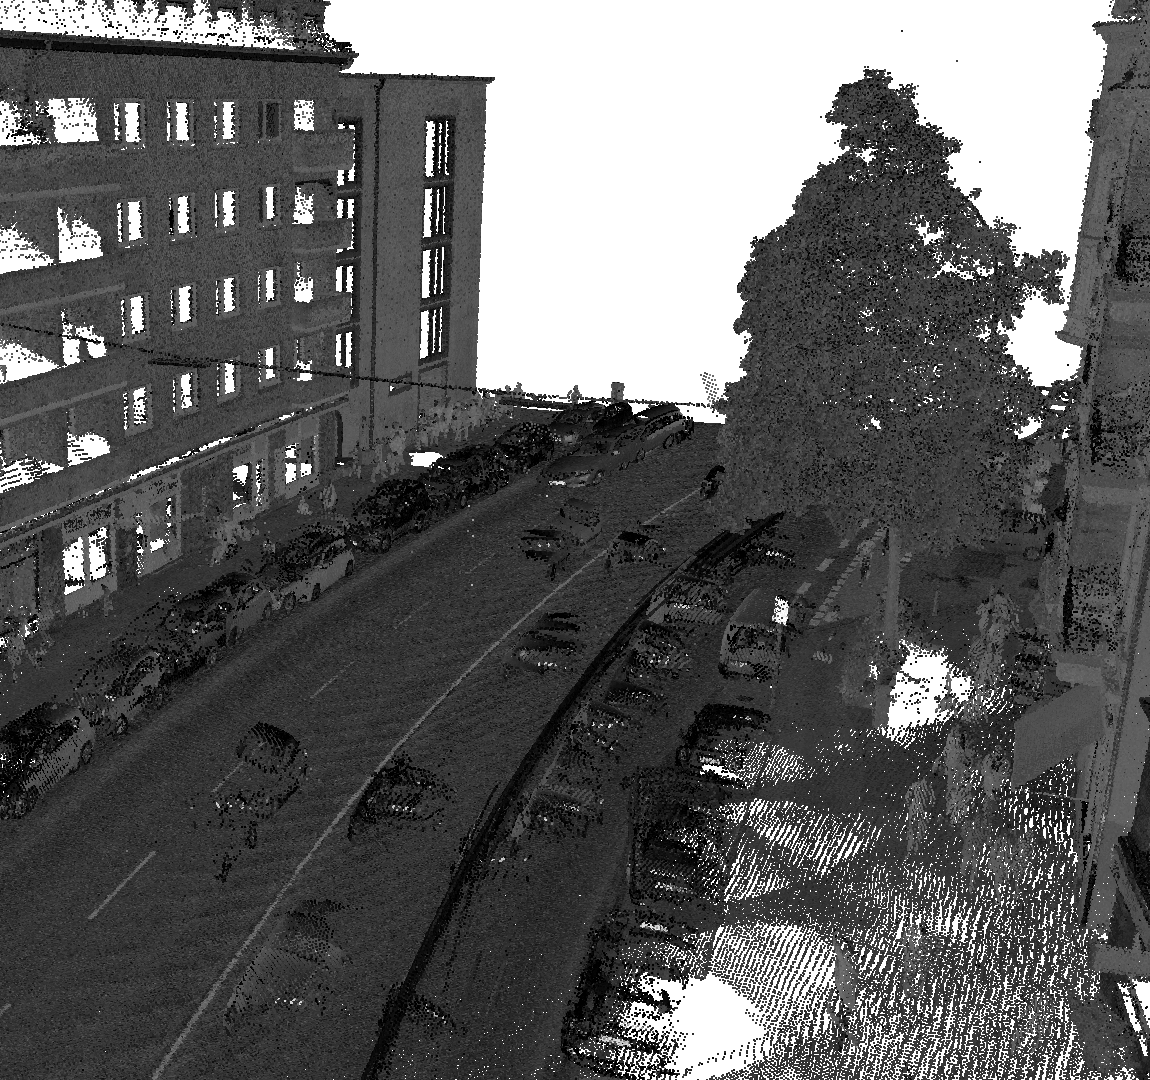
\includegraphics[width=0.327\textwidth]{graphics/mm_plain_view}}
    \hfill
    \subcaptionbox{\label{fig:test3b}Airborne-LiDAR}{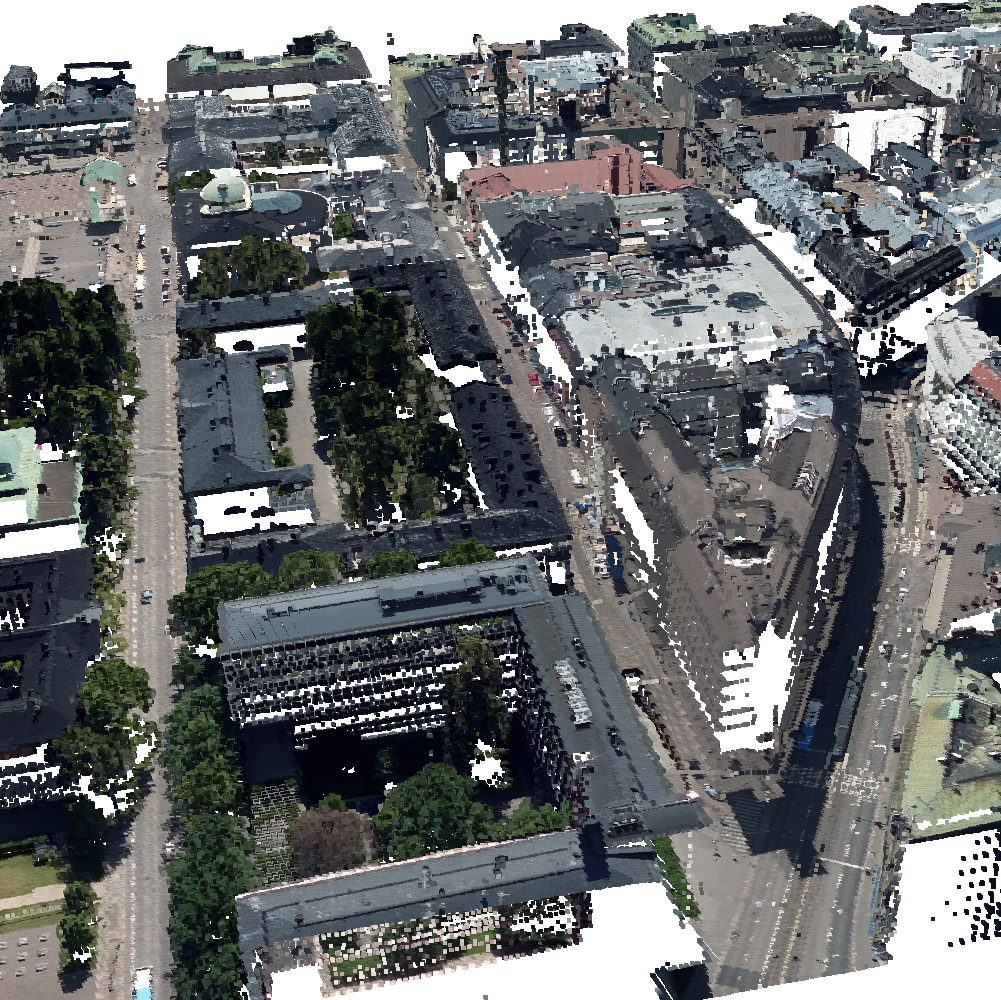
\includegraphics[width=0.327\textwidth]{graphics/air_plain_view}}
    \hfill
    \subcaptionbox{\label{fig:test3c}Photogrammetrie}{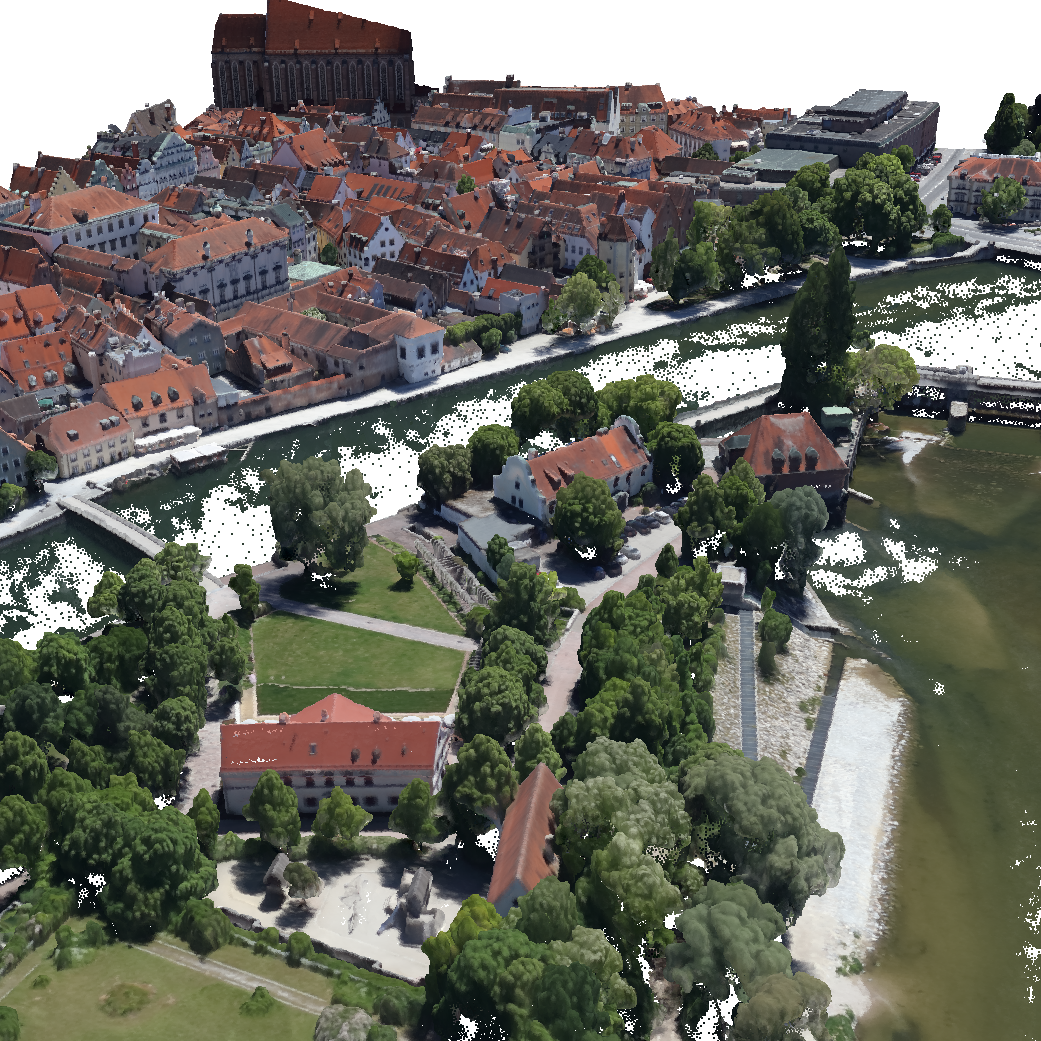
\includegraphics[width=0.327\textwidth]{graphics/photo_view}}
    \caption{3D-Punktwolken verschiedener europäischer Städte.}
    \label{fig:example_pcs}
\end{figure}

\subsection*{Laserscanner (LiDAR)}
LiDAR-Scanner \citep{Collis-1970} verwenden Laserstrahlen, um eine Umgebung abzutasten. Wenn diese Strahlen auf eine Oberfläche treffen, werden sie reflektiert und wieder in Richtung Scanner zurückgeworfen. Der LiDAR-Scanner misst die Zeitdifferenz zwischen Aussenden des Strahls und Regristrierung der Reflexion und kann so die Position des Reflexionspunktes ermitteln. Es können so aber auch andere Oberflächeneigenschaften erfasst werden, wie beispielsweise die Helligkeit der abgetasteten Oberfläche (der so genannte Intensitätswert). Der Scanner erfasst die Oberflächen dabei jedoch nicht als Ganzes, sondern generiert selbst nur 3D-Punkte, welche in 3D-Punktwolken abgespeichert werden. Um später aus diesen Punkten Klassifizierungs- und Objektinformationen ableiten zu können, sind verschiedene Verfahren und Algorithmen nötig.

\subsection*{Photogrammetrie}
Bei der Photogrammetrie \citep{Linder-2009, Remondino.ElHakim-2006} werden aus 2D-Daten wie Bildern und Videos Tiefeninformationen der abgebildeten Objekte errechnet. Dabei stützt man sich vor allem auf das Prinzip der Stereoskopie aus der Biologie. Menschen beispielsweise sind in der Lage die Position von Objekten im Raum zu bestimmen, da diese Objekte in den Blickfeldern der einzelnen Augen leicht versetzt sind. Die Photogrammetrie nutzt auf gleiche Weise eine Anzahl an versetzt aufgenommenen Bildern, um so die Distanz von Objekten zur Kamera zu bestimmen. Die so gewonnenen 3D-Darstellungen von Objekten werden dann in 3D-Punktwolken konvertiert, welche im Kontext der Projekttätigkeit bearbeitet werden.

\subsection*{Mobile-Mapping}
\textit{Mobile Mapping} ist eine Spezialform der 3D-Punktwolken-Generierung durch LiDAR-Scanner, wobei der Laserscanner auf einer mobilen, sich bewegenden Plattform montiert ist \citep{Puente.etal-2013}. Als Basis dienen hierfür meist verschiedene Arten von Boden- und Luftfahrzeugen wie beispielsweise Autos oder Drohnen. Für die Aufnahme von Straßenzügen eignen sich hier insbesondere \textit{Mobile-Mapping}-Fahrzeuge \citep{Ellum.ElSheimy-2002}, welche die Straße und die lokale Umgebung sehr präzise erfassen. Ein solches Fahrzeug der Stadt Essen ist in Abbildung \ref{fig:mm_vehicle} dargestellt.

\begin{figure}[!ht]
  \centering
  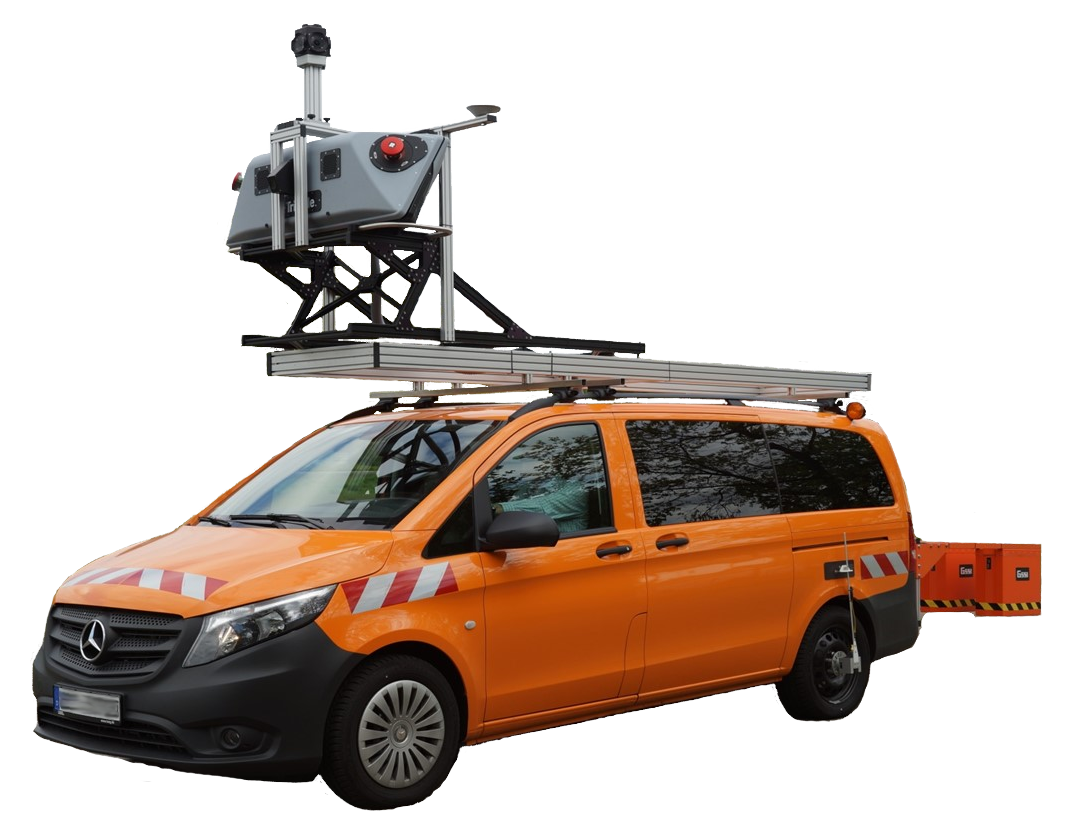
\includegraphics[width=0.5\textwidth]{graphics/mm_vehicle}
  \caption{Mobile-Mapping-Fahrzeug der Stadt Essen.}
  \label{fig:mm_vehicle}
\end{figure}

\subsection*{Deep-Learning}
Unter \textit{Deep Learning} versteht man das Anwenden eines lernenden mehrschichtigen künstlichen neuronalen Netzes auf eine komplexe Problemstellung, welche sich meist nur schwer oder auch gar nicht mit nicht lernenden Algorithmen lösen lässt. Dabei orientiert man sich stark an der Funktionsweise von Nervenzellen im menschlichen Gehirn. Häufig kommt dabei sogenanntes \textit{Supervised Learning} zum Einsatz, bei dem mit Hilfe von zuvor manuell erstellten Trainings- und Testdaten ein neuronales Netz zunächst trainiert und dann mit Hilfe der Testdaten evaluiert wird. Ein so trainiertes neuronales Netz kann anschließend verwendet werden, um auf neuen Daten die zuvor antrainierten Berechnungen durchzuführen.

\subsection*{Das \textit{PCNN}-Framework}

Mit dem am Lehrstuhl entwickelten \textit{PCNN}-Framework können mithilfe von \textit{JSON}-Dateien konfigurierte neuronale Netze auf 3D-Punktwolken trainiert werden. Dazu implementiert das Framework einige Architekturen von \textit{Deep-Learning}-Modellen und Funktionalitäten, um 3D-Punktwolken vorzuverarbeiten oder semantische Segmentierungen auf ihnen ausführen zu lassen.

\subsection*{Das \textit{PCR}-Framework}

Das ebenfalls am Lehrstuhl entwickelte \textit{PCR}-Framework implementiert eine Reihe von Analyse- und Manipulationsverfahren für Punktdaten. Diese Algorithmen lassen sich sowohl auf einer grafischen Oberfläche konfigurieren als auch als Kommandozeilentool mithilfe einer Konfigurations-\textit{JSON}-Datei verwenden. So können beispielsweise geometrische Klassifikationsalgorithmen und Normalen- oder Teilmengenberechnungen auf 3D-Punktwolken ausgeführt werden.

\section{Schwerpunkte des Bachelorprojekts}

Im Projektverlauf sind diverse Analyse- und Verarbeitungsverfahren für 3D-Punktwolken sowie eine webbasierte Plattform zur Bündelung dieser und bereits vorhandener Funktionalitäten entstanden.
Die einzelnen Schwerpunkte des Bachelorprojekts werden im Folgenden kurz vorgestellt.

\subsection{Fingerabdrücke von 3D-Punktwolken}

Da 3D-Punktwolken häufig aus Millionen von Punkten bestehen, können aufwändige, punktspezifische Verarbeitungsverfahren sehr zeitintensiv sein. Es existieren darüber hinaus allerdings auch Verfahren, welche nicht punktspezifisch sind, sondern lediglich ein Ergebnis für die gesamte 3D-Punktwolke erzeugen. Um den Zeitaufwand solcher Verfahren zu reduzieren, kann zunächst der Fingerabdruck einer 3D-Punktwolke berechnet werden, der nur einen Bruchteil der ursprünglichen Größe aufweist. Dieser Fingerabdruck wird dann anstelle der 3D-Punktwolke für weitere Verarbeitungsschritte verwendet. Dabei gibt es verschiedene Möglichkeiten, wie ein solcher Fingerabdruck erstellt werden kann. In diesem Projekt besteht der Fingerabdruck aus einer Sammlung von Histogrammen, die \textit{PCFP} genannt wird. Der \textit{PCFP} wird dann verwendet, um Operationen wie eine Punktwolkenklassifizierung mit einem tiefen neuronalen Netz oder eine Parameterschätzung für \textit{Machine-Learning}-Modelle auf der Grundlage von Parametern ähnlicher 3D-Punktwolken durchzuführen. So können zum Beispiel Parameter und Modelle, welche auf eine Straßenzustandserkennung optimiert sind, schnell auch für eine andere 3D-Punktwolke verwendet werden, um mögliche Straßenschäden mit wenig Verzögerung aufzudecken.

\subsection{Bodenerkennungsalgorithmen und Deep-Learning auf Punktwolken}

Für eine schnelle und gute Schätzung von Parametern für verschiedene Analysen auf noch ungesehenen 3D-Punktwolken benötigen wir einen Satz an Parametern und Modellen, die auf bereits vorhandenen 3D-Punktwolken aufwändig berechnet oder trainiert werden müssen. Dafür haben wir Mechanismen entwickelt, die geometrische Eigenschaften von 3D-Punktwolken extrahieren und daraus mittels Heuristiken Eingabeparameter für beispielsweise eine Bodenerkennung ermitteln können. Daneben haben wir eine genetische Hyperparameteroptimierung für \textit{Deep-Learning}-Modelle zur semantischen Segmentierung auf 3D-Punktwolken implementiert, damit wir für 3D-Punktwolken mit vorannotierten Klassen die besten Trainingsparameter finden und so auf unannotierten 3D-Punktwolken optimierte Modelle anwenden können.

\subsection{Straßenzustandserkennung}

Moderne Laserscanner, die auf einem entsprechenden Fahrzeug montiert sind, bieten höchste Präzision und können Straßenzüge millimetergenau erfassen. Damit wird eine automatische Analyse dieser Straßen-Punktwolken motiviert, die auch kleine Schäden wie Schlaglöcher und feine Ausbesserungen wie Flickstellen identifizieren soll. Herausfordernd sind dabei vor allem die hohe Punktdichte und die unregelmäßige Natur solcher Schäden. In diesem Projektteil werden zwei Ansätze getestet und verglichen: ein klassischer \textit{Machine-Learning}-Ansatz mit der Extraktion manuell definierter Features sowie ein moderner \textit{Deep-Learning}-Ansatz, der aber ebenfalls direkt auf Punktmengen arbeitet.

\subsection{Entwicklung einer webbasierten Plattform}

Die effektive Analyse, Verarbeitung und Visualisierung von 3D-Punktwolken erfordert aktuell häufig komplexe Verarbeitungsprozesse und sehr leistungsstarke Hardware. Durch die während des Projekts entwickelte webbasierte Plattform werden verschiedene Anwendungen in einem einzelnen Projekt gebündelt und um eine hohe Skalierbarkeit mittels Lastenverteilung auf viele Rechner in einem \textit{Cluster} erweitert. Dies ermöglicht auf der einen Seite eine Vereinfachung der Verarbeitungsprozesse, was die Plattform auch für Nutzer mit weniger fundiertem Fachwissen nutzbar macht. Auf der anderen Seite wird so auch eine Beschleunigung bei der Verarbeitung vieler 3D-Punktwolken durch die Verteilung der nötigen Berechnungsschritte auf alle verfügbaren Rechner erzielt.

\section{Einordnung in den Projektkontext}

Im Zuge dieser Arbeit sind unter \textit{Punktwolken} immer 3D-Punktwolken zu verstehen. Die potenzielle Menge an Anwendungsfällen solcher Punktwolken ist groß. Entsprechend sollte auch die Webplattform neben ihrer einfachen und intuitiven Bedienung bereits nützliche Funktionalität bieten. Abseits von zumindest teilweise ausgereiften Verfahren wie der Bodenerkennung bot sich die Erkennung von Straßenschäden in Punktwolken aus zweierlei Gründen an:
\begin{itemize}
    \item Die Genauigkeit des \textit{Mobile Mapping} von Bodenfahrzeugen erlaubt es - im Gegensatz zu eher groberen aus der Luft aufgenommenen Punktwolken - grundsätzlich, auch kleinere und feinere Schäden oder sonstige Objekte von Interesse zu identifizieren.
    \item Die Suche nach Straßenschäden durch etwa Straßenbaubehörden ist meist noch immer eine manuelle Aufgabe. Ob die Schäden bei einer Fahrt durch die Stadt durch bloßen Blick gesichtet werden oder bei Ansehen von aufgenommenen Videos der Fahrbahnoberfläche: Solche Methoden sind personal- und zeitaufwändig und naturgemäß trotzdem fehleranfällig.
\end{itemize}
Diese Anwendung kann also für einige Nutzer der Plattform sinnvoll sein. Entsprechend wurde sie darin integriert und kann durch einfache Bestätigung gestartet werden. Wie bei anderen Aktionen auf Punktwolken werden auch in diesem Fall die notwendigen Schritte gestartet und, wo immer möglich, verteilt auf verschiedenen Rechnern ausgeführt.

\section{Struktur der Arbeit}

Die restliche Arbeit gliedert sich wie folgt: In Kapitel 2 werden verwandte Arbeiten vorgestellt, anschließend folgt in Kapitel 3 ein Überblick zu verwendeten Systemen und betrachteten Klassen. Kapitel 4 behandelt das beiden Ansätzen gemeine \textit{Preprocessing}, während die Kapitel 5, 6 und 7 Erläuterungen zur Featureberechnung, dem \textit{Uniqueness}-Konzept und \textit{Predictions} im eigenen \textit{Feature-Extraction}-Ansatz beinhalten. Kapitel 8 thematisiert die Arbeitsweise und Bedienung des \textit{Deep-Learning}-Ansatzes, wonach in Kapitel 9 das genutzte \textit{Postprocessing} erklärt wird. In Kapitel 10 wird eine Evaluierung der beiden getesteten Ansätze vorgenommen. Das abschließende Kapitel 11 stellt ein Fazit zu den Ergebnissen und gibt einen Ausblick auf mögliche Verbesserungen und Erweiterungen.